%iffalse
\let\negmedspace\undefined
\let\negthickspace\undefined
\documentclass[journal,12pt,onecolumn]{IEEEtran}
\usepackage{cite}
\usepackage{amsmath,amssymb,amsfonts,amsthm}
\usepackage{algorithmic}
\usepackage{graphicx}
\usepackage{textcomp}
\usepackage{xcolor}
\usepackage{txfonts}
\usepackage{listings}
\usepackage{enumitem}
\usepackage{mathtools}
\usepackage{gensymb}
\usepackage{comment}
\usepackage[breaklinks=true]{hyperref}
\usepackage{tkz-euclide} 
\usepackage{listings}
\usepackage{gvv}                                        
% \usepackage{gvv}  
\usepackage[latin1] {inputenc}
\usepackage{xparse}
\usepackage{color}                                            
\usepackage{array}                                            
\usepackage{longtable}                                       
\usepackage{calc}                                             
\usepackage{multirow}
\usepackage{multicol}
\usepackage{hhline}                                           
\usepackage{ifthen}                                           
\usepackage{lscape}
\usepackage{tabularx}
\usepackage{array}
\usepackage{float}
\newtheorem{theorem}{Theorem}[section]
\newtheorem{problem}{Problem}
\newtheorem{proposition}{Proposition}[section]
\newtheorem{lemma}{Lemma}[section]
\newtheorem{corollary}[theorem]{Corollary}
\newtheorem{example}{Example}[section]
\newtheorem{definition}[problem]{Definition}
\newcommand{\BEQA}{\begin{eqnarray}}
\newcommand{\EEQA}{\end{eqnarray}}
\usepackage{float}
%\newcommand{\define}{\stackrel{\triangle}{=}}
\theoremstyle{remark}
\usepackage{ circuitikz }
%\newtheorem{rem}{Remark}
% Marks the beginning of the document
\begin{document}
\title{GATE BT 2017}
\author{EE25BTECH11044 - Pappula Sai Hasini}
\maketitle
\renewcommand{\thefigure}{\theenumi}
\renewcommand{\thetable}{\theenumi}
%GATE BT 2017
\begin{enumerate}

 \item 

an enzyme catalyses a reaction by
 
 \begin{enumerate}
    \item decreasing the energy of the substrate 
    \item decreasing the activation energy of the reaction 
    \item decreasing the product stability
    \item increasing the activation barrier of the reaction
 \end{enumerate}
 \hfill (GATE BT 2017)
 \item 

 Natural protiens are composed primarily of $20$ $ \alpha $
amino acids. Which of the following statements is true for any of these amino acids in a solution of pH $1.5$?

\begin{enumerate}
    \item only the amino group is ionized
    \item only the carboxylic group is ionized 
    \item both amino and carboxylic groups are ionized
    \item both amino and carboxylic groups are neutral
\end{enumerate}
\hfill (GATE BT 2017)
\item 

which one of the following organisms is an indicator of fecal contamination?

\begin{enumerate}
    \item Escherichia cell
    \item Streptococus lactis
    \item Bacillus subtilis
    \item Lactobacillus acidophilus
\end{enumerate}
\hfill (GATE BT 2017)
\item 

The surface area (in $m^2$) of the largest sphere that can fit into a hollow cube with edges of length $1$ meter is 
\hfill (GATE BT 2017)

\item 

In a thin layer chromatography experiment using a silical gel plate, a compund showed migration of $12.5$cm and the solvent front showed migration of $18$cm . The Rf value for the compound is 
\hfill (GATE BT 2017)

\item 

\[
\lim_{x\to 0}\frac{\sin x}{x}=1
\]
\hfill (GATE BT 2017)

\item Which one of the following mechanisms is used by human pathogens to evade host immune responses?
\begin{enumerate}
    \item Somatic hypermutation
    \item Antibody production
    \item Antigenic variation
    \item Complement activation
\end{enumerate}
\hfill(GATE BT 2017)

\item If the nucleotide composition (\%) of a viral genome is $A=10$, $U=20$, $C=40$, and $G=30$, which one of the following is this genome?
\begin{enumerate}
    \item Double stranded RNA
    \item Single stranded RNA
    \item Single stranded DNA
    \item Double stranded DNA
\end{enumerate}
\hfill (GATE BT 2017)

\item Which one of the following techniques can be used to determine the structure of a 15 kDa globular protein at atomic resolution?
\begin{enumerate}
    \item Raman spectroscopy
    \item IR spectroscopy
    \item UV spectroscopy
    \item NMR spectroscopy
\end{enumerate}
\hfill (GATE BT 2017)

\item Assertion [a]: Gram negative bacteria show staining with saffranin. \\
Reason [r]: Gram negative bacteria have an outer membrane with lipopolysaccharides.
\begin{enumerate}
    \item Both [a] and [r] are true and [r] is the correct reason for [a].
    \item Both [a] and [r] are true but [r] is not the correct reason for [a].
    \item Both [a] and [r] are false.
    \item [a] is true but [r] is false.
\end{enumerate}
\hfill (GATE BT 2017)

\item Enzyme-linked immunosorbent assay (ELISA) is used for
\begin{enumerate}
    \item quantifying antibody levels in blood
    \item determining the molecular weight of an antigen
    \item purifying proteins from biological fluids
    \item determining the molecular weight of an antibody
\end{enumerate}
\hfill (GATE BT 2017)

\item Macrophages eliminate pathogenic bacteria upon activation by
\begin{enumerate}
    \item NK cells
    \item basophils
    \item CD4+ T cells
    \item plasma cells
\end{enumerate}
\hfill (GATE BT 2017)

\item If a protein contains four cysteine residues, the number of different ways they can simultaneously form two intra-molecular disulphide bonds is  
\hfill (GATE BT 2017)

\item Secretory proteins synthesized by ER-associated ribosomes traverse through
\begin{enumerate}
    \item mitochondria
    \item peroxisomes
    \item the Golgi apparatus
    \item the nucleus
\end{enumerate}
\hfill (GATE BT 2017)

\item For $y=f(x)$, if $\dfrac{d^{2}y}{dx^{2}}=0$, $\dfrac{dy}{dx}=0$ at $x=0$, and $y=1$ at $x=1$, the value of $y$ at $x=2$ is   

\hfill (GATE BT 2017)

\item During protein synthesis, tRNAs are NOT involved in
\begin{enumerate}
    \item termination
    \item elongation 
    \item  charging 
    \item initiation   
     \end{enumerate}
\hfill (GATE BT 2017)

\item In eukaryotes, cytokinesis is inhibited by  
\begin{enumerate}
    \item cytochalasin D
    \item vinblastine
    \item nocodazole
    \item colchicine
\end{enumerate}
\hfill (GATE BT 2017)

\item A proto-oncogene is suspected to have undergone duplication in a certain type of cancer. Of the following techniques, which one would verify the gene duplication?  
\begin{enumerate}
    \item Northern blotting
    \item Southern blotting
    \item South western blotting
    \item Western blotting
\end{enumerate}
\hfill (GATE BT 2017)

\item A polymerase chain reaction (PCR) was set up with the following reagents: DNA template, \textit{Taq} polymerase, buffer, dNTPs, and $Mg^{2+}$. Which one of the following is missing in the reaction mixture?
\begin{enumerate}
    \item Helicase
    \item Single-stranded binding proteins
    \item Primers
    \item Reverse transcriptase
\end{enumerate}
\hfill (GATE BT 2017)

\item
An enzymatic reaction exhibits Michaelis--Menten kinetics. For this reaction, on doubling the concentration of enzyme while maintaining \([S] \gg [E_{0}]\), the maximum velocity \(V_{\max}\) is doubled, while the Michaelis constant \(K_m\) remains unchanged.

\begin{enumerate}
    \item both $K_{m}$ and $V_{\max}$ will remain the same.
    \item $K_{m}$ will remain the same but $V_{\max}$ will increase.
    \item $K_{m}$ will increase but $V_{\max}$ will remain the same.
    \item both $K_{m}$ and $V_{\max}$ will increase.
\end{enumerate}
\hfill (GATE BT 2017)

\item A 5 liter chemostat is fed fresh medium at $0.2$ liters/minute having a substrate concentration of $25$ grams/liter. At steady state, the outgoing stream has substrate concentration of $2.5$ grams/liter. The rate of consumption (grams/liter/minute) of the substrate in the reactor is \rule{2cm}{0.4pt}.
\hfill (GATE BT 2017)

\item The transcription factor X binds a 10 base pair DNA stretch. In the DNA of an organism, 
X was found to bind at 20 distinct sites. An analysis of these 20 binding sites showed the following distribution:

\begin{figure}[h!]
    \centering
    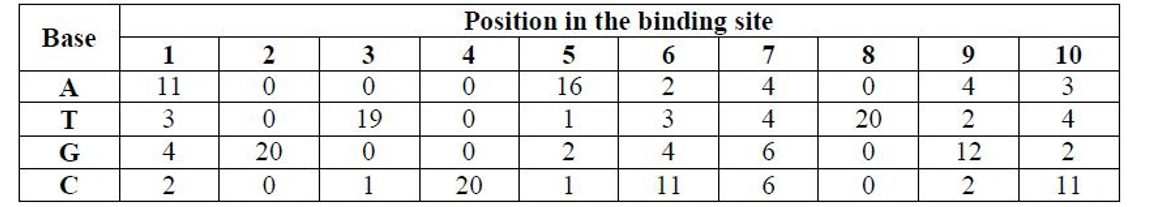
\includegraphics[width=\columnwidth]{figs/table.png} 
    \caption{Distribution of bases at each position of the binding site}
    \label{fig:binding-site}
\end{figure}

What is the consensus sequence for the binding site of X?

\begin{enumerate}
    \item NGTCNNNTNN
    \item AGTCACNTGC
    \item CACCTANCTG
    \item ANNNACGNGC
\end{enumerate}
\hfill (GATE BT 2017)

\item A bacterium has a genome of size $6$ million base pairs. If the average rate of DNA synthesis is $1000$ base pairs/second, the time taken (in minutes) for replication of the genome will be \rule{2cm}{0.4pt}.
\hfill (GATE BT 2017)

\item At the transcription start site of a gene, any of the four nucleotides can occur with equal probability $p$. The Shannon Entropy $S$, given by $S=-\sum_{i=1}^{4} p_{i}\ln p_{i}$, for this start site is \rule{2cm}{0.4pt}.
\hfill (GATE BT 2017)

\item The distribution of marks scored by a large class in an exam can be represented as a normal distribution with mean $\mu$ and standard deviation $\sigma$. In a follow-up exam in the same class, everyone scored 5 marks more than their respective score in the earlier exam. For this follow-up exam, the distribution of marks can be represented as a normal distribution with mean $\mu_{2}$ and standard deviation $\sigma_{2}$. Which one of the following is correct?
\begin{enumerate}
    \item $\mu=\mu_{2};\ \sigma>\sigma_{2}$
    \item $\mu<\mu_{2};\ \sigma>\sigma_{2}$
    \item $\mu>\mu_{2};\ \sigma<\sigma_{2}$
    \item $\mu<\mu_{2};\ \sigma=\sigma_{2}$
\end{enumerate}
\hfill (GATE BT 2017)

Which one of the following graphs represents the kinetics of protein precipitation by addition of ammonium sulphate? On the Y-axis, [Protein] represents the concentration of free protein in solution.

\begin{enumerate}
    \item \includegraphics[width=0.4\columnwidth]{figs/oA.png}
    \item \includegraphics[width=0.4\columnwidth]{figs/oB.png}
    \item \includegraphics[width=0.4\columnwidth]{figs/oC.png}
    \item \includegraphics[width=0.4\columnwidth]{figs/oD.png}
\end{enumerate}
\hfill (GATE BT 2017)

\item The angle (in degrees) between the vectors $\vec{x}=\hat{i}-\hat{j}+2\hat{k}$ and $\vec{y}=2\hat{i}-\hat{j}-1.5\hat{k}$ is 
\hfill (GATE BT 2017)

\item Match the proteins in Group I with cellular processes in Group II.

\begin{tabbing}
\hspace{4cm} \= \kill
Group I \> Group II \\
P.\ p53 \> 1.\ DNA packaging \\
Q.\ Lysozyme \> 2.\ Apoptosis \\
R.\ Tubulins \> 3.\ Hydrolysis of polysaccharides \\
S.\ Histones \> 4.\ Chromosome segregation \\
\end{tabbing}

\begin{enumerate}
    \item P-4, Q-2, R-3, S-1
    \item P-2, Q-3, R-1, S-4
    \item P-4, Q-3, R-1, S-2
    \item P-2, Q-3, R-4, S-1
\end{enumerate}
\hfill (GATE BT 2017)

\item Match the organisms in Column I with the characteristics in Column II.

\begin{tabbing}
\hspace{4cm} \= \kill
Column I \> Column II \\
P.\ \textit{Methanococcus} \> 1.\ Halophile \\
Q.\ \textit{Dunaliella} \> 2.\ Acidophile \\
R.\ \textit{Sulfolobus} \> 3.\ Mesophile \\
S.\ \textit{Escherichia} \> 4.\ Barophile \\
\end{tabbing}

\begin{enumerate}
    \item P-4, Q-3, R-2, S-1
    \item P-3, Q-2, R-4, S-1
    \item P-2, Q-1, R-4, S-3
    \item P-4, Q-1, R-2, S-3
\end{enumerate}
\hfill (GATE BT 2017)

\item 
secretory protiens synthesised by ER-associated ribosomes transverse through

\begin{enumerate}
    \item mitochondria
    \item peroxisomes
    \item the Golgi apparatus
    \item the nucleus
\end{enumerate}
\hfill (GATE BT 2017)

\item
The circular dichroism spectra of three proteins P, Q, and R are shown below:

\begin{figure}
  \centering
  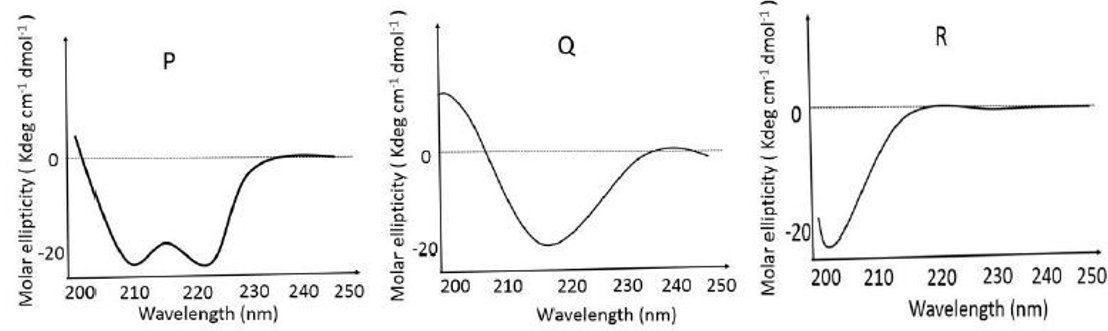
\includegraphics[width=\columnwidth]{figs/cd_spectra.png}
  \caption{CD spectra of proteins P, Q, and R}
  \label{fig:cd_spectra}
\end{figure}

Choose the correct combination.

\begin{enumerate}
  \item P: $\alpha$-helix,\; Q: $\beta$-sheet,\; R: Random coil
  \item P: $\beta$-sheet,\; Q: $\alpha$-helix,\; R: Random coil
  \item P: $\alpha$-helix,\; Q: Random coil,\; R: $\beta$-sheet
  \item P: Random coil,\; Q: $\alpha$-helix,\; R: $\beta$-sheet
\end{enumerate}

\item Which one of the following amino acids has three ionizable groups?

\begin{enumerate}
    \item Glycine
    \item Leucine
    \item Valine
    \item Lysine
\end{enumerate}
\hfill (GATE BT 2017)

\item
Consider an infinite number of cylinders. The first cylinder has a radius of $1$ meter and height of $1$ meter. The second one has a radius of $0.5$ meter and height of $0.5$ meter. Every subsequent cylinder has half the radius and half the height of the preceding cylinder. The sum of the volumes (in cubic meters) of these infinite number of cylinders is 

Given data: $\pi = 3.14$.
\hfill (GATE BT 2017)

\item
The concentration (in micromolar) of NADH in a solution with $A_{340}=0.50$ is 

Given data: Path length $=1cm$; Molar extinction coefficient of NADH $\varepsilon_{340}=6220\ {M^{-1}\,cm^{-1}}$.
\hfill (GATE BT 2017)

\item
The specific activity of an enzyme in a crude extract of \textit{E.\ coli} is $9.5$ units/mg of protein. The specific activity increased to $68$ units/mg of protein upon ion-exchange chromatography. The fold purification is 
\hfill (GATE BT 2017)

\item Which one of the following organisms is responsible for crown gall disease in plants?  

\begin{enumerate}
    \item Xanthomonas campestris
    \item Rhizobium etli
    \item Agrobacterium tumefaciens
    \item Erwinia stewartii
\end{enumerate}
\hfill (GATE BT 2017)

\item In eukaryotes, cytokinesis is inhibited by  
\begin{enumerate}
    \item cytochalasin D
    \item vinblastine
    \item nocodazole
    \item colchicine
\end{enumerate}
\hfill (GATE BT 2017)

\item The value of $c$ for which the following system of linear equations has an infinite number of solutions is \rule{2cm}{0.4pt}.
\[
\begin{bmatrix}1 & 2\\ 1 & 2\end{bmatrix}
\vec{x} =
\begin{bmatrix}c\\ 4\end{bmatrix}
\]
\hfill (GATE BT 2017)

\item Match the plant hormones in Column I with functions in Column II

\begin{tabbing}
Column I \hspace{4cm} \= Column II \\ 
P. Gibberellic acid \= 1. Seed and bud dormancy \\ 
Q. Zeatin \= 2. Fruit ripening \\ 
R. Ethylene \= 3. Delaying leaf senescence \\ 
S. Abscisic acid \= 4. Regulation of plant height \\ 
\end{tabbing}

\begin{enumerate}
    \item P-4, Q-3, R-2, S-1
    \item P-4, Q-2, R-3, S-1
    \item P-3, Q-1, R-2, S-4
    \item P-2, Q-1, R-4, S-3
\end{enumerate}
\hfill (GATE BT 2017)

\item For an \textit{E.\ coli} culture in the exponential phase of growth, optical density ($\mathrm{OD}_{540}$) is $0.3$ at $2$ hours and $0.6$ at $4$ hours. Assuming that the measured OD is linearly proportional to the number of \textit{E.\ coli} cells, the growth rate (per hour) for this culture is 
\hfill (GATE BT 2017)

\item 

The interaction energy $E$ between two spherical particles is plotted as a function of the distance $r$ 
between them. When $r<a$, where $a$ is a constant, the net force between the spherical particles is 
repulsive. When $r \geq a$, they attract via van der Waals attraction. Which one of the following plots 
correctly represents the interaction energy between the above two particles?

\begin{enumerate}
    \item 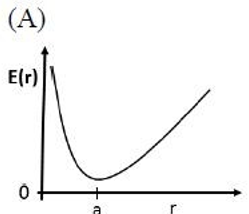
\includegraphics[width=0.22\columnwidth]{figs/A.png}
    \item 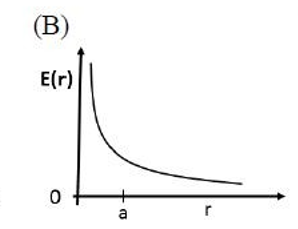
\includegraphics[width=0.22\columnwidth]{figs/B.png}
    \item 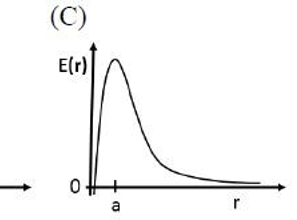
\includegraphics[width=0.22\columnwidth]{figs/C.png}
    \item 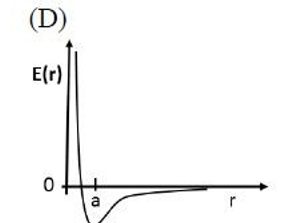
\includegraphics[width=0.22\columnwidth]{figs/D.png}
\end{enumerate}


\item The genome is diploid at the end of which phases of a human mitotic cell cycle?
\begin{enumerate}
    \item G2 \& S
    \item G1 \& M
    \item M \& S
    \item G1 \& G2
\end{enumerate}
\hfill (GATE BT 2017)

\item 
An immunocompetent person becomes infected with a pathogenic strain of bacteria. 
Which one of the following graphs correctly depicts bacterial load in this person over time
\begin{figure}
    \centering
    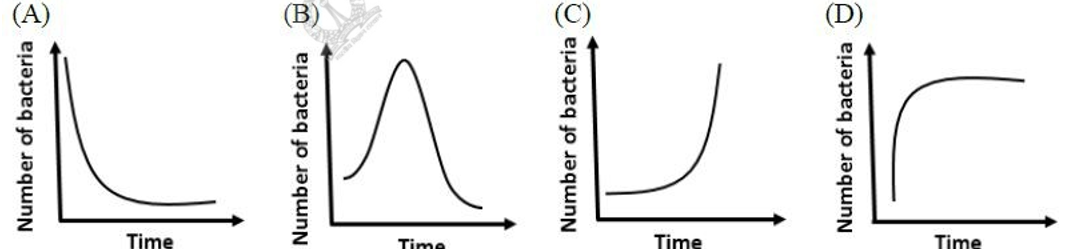
\includegraphics[width=\columnwidth]{figs/bacteria_load.png}
\end{figure}

\hfill (GATE BT 2017)
\item A recombinant protein is to be expressed under the control of the lac promoter and operator in a strain of \textit{E.\ coli} having the genotype $lacI^{+}\ crp^{+}$. Even in the absence of inducer IPTG, low levels of expression of the recombinant protein are seen (leaky expression). Which one of the following should be done to minimize such leaky expression?

\begin{enumerate}
    \item Addition of lactose to the medium
    \item Removal of all glucose from the medium
    \item Addition of excess glucose to the medium
    \item Addition of \textit{allo}-lactose to the medium
\end{enumerate}
\hfill (GATE BT 2017)

\item
Shown below is a plasmid vector (P) and an insert (Q). The insert was cloned into the \textit{BamHI} site of the vector. The recombinant plasmid was isolated and digested with \textit{BamHI} or \textit{XhoI}. The results from the digestion experiments are shown in (R). 

\begin{figure}
    \centering
    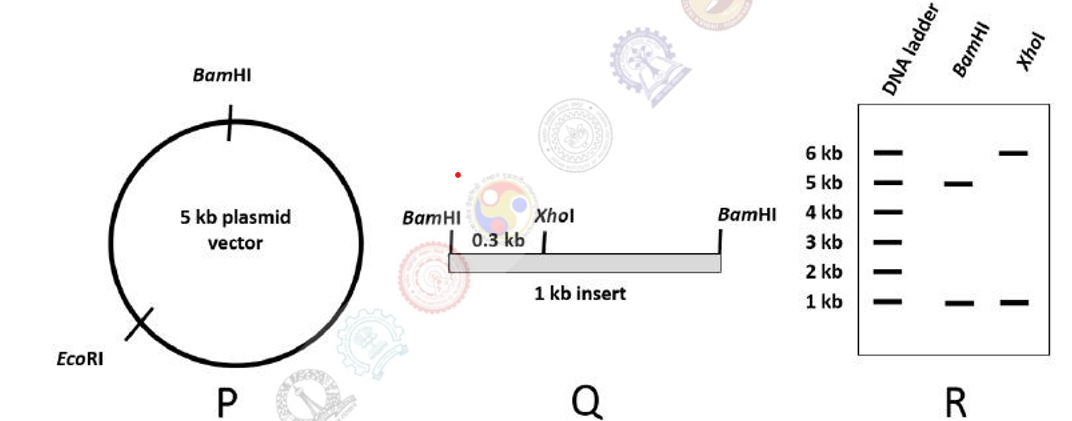
\includegraphics[width=\columnwidth]{figs/vector_question.png}
\end{figure}


Which one of the following explains the digestion results shown in (R)?

\begin{enumerate}
    \item The insert did not ligate to the vector.
    \item One copy of the insert ligated to the vector.
    \item The insert ligated to the vector as two tandem copies.
    \item The insert ligated to the vector as two copies but not in tandem.
\end{enumerate}
\hfill (GATE BT 2017)

\item Which one of the following CANNOT be a recognition sequence for a Type II restriction enzyme?

\begin{enumerate}
\item GAATTC
\item AGCT
\item GCGGCCGC
\item ATGCCT
\end{enumerate}

\item
Which one of the given options is appropriate to fill the blank?

\begin{enumerate}
    \item starve
    \item reject
    \item feast
    \item deny
\end{enumerate}

\hfill (GATE BT 2017)

\begin{figure}
\centering
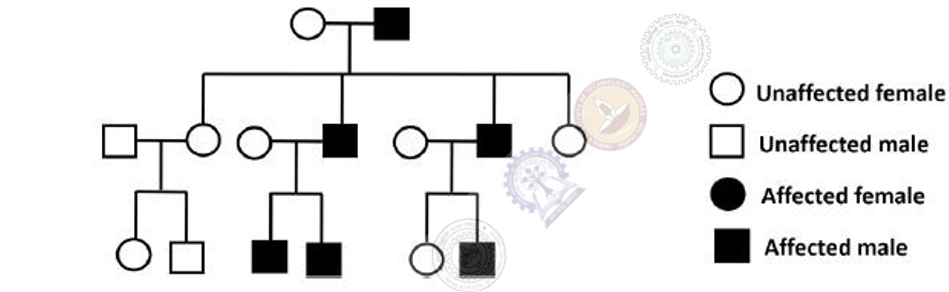
\includegraphics[width=\columnwidth]{figs/disease.png}
\caption{Pedigree for an inheritable disease.}
\label{fig:gate2017-pedigree}
\end{figure}

\item A pedigree of an inheritable disease is shown in Fig.~\ref{fig:gate2017-pedigree}. This inheritable disease is

\begin{enumerate}
\item X-linked dominant
\item X-linked recessive or Y-linked
\item only Y-linked
\item only X-linked recessive
\end{enumerate}

\hfill (GATE BT 2017)

\item If the chemical composition of proteins in an organism is $CH_{1.5}O_{0.3}N_{0.3}S_{0.004}$, the mass percentage of carbon in the proteins is 

Given data: Atomic weights (Da) of C = 12, H = 1, O = 16, N = 14, and S = 32.

\hfill (GATE BT 2017)

\item For the probability density $P(x)=0.5e^{-0.5x}$, the integral $\int_{0}^{\infty} P(x)\,dx$ is 

\hfill (GATE BT 2017)

\item A zero-order liquid phase reaction $A \rightarrow B$ is being carried out in a batch reactor with $k = 10^{-3}$ mol/min. If the starting concentration of $A$ is $0.1$ moles/liter, the time (in minutes) taken by the system before $A$ is exhausted in a $100$ liter reactor is \underline{\hspace{2cm}}.

\hfill (GATE BT 2017)

\item \textit{EcoRI} restriction sites on a 10 kb DNA fragment are shown below.
\begin{figure}
    \centering
    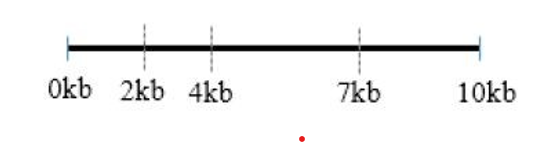
\includegraphics[width=\columnwidth]{figs/fragment .png}
    \caption{Map of \textit{EcoRI} sites on a 10 kb fragment}
    \label{fig:ecoRI-partial}
\end{figure}

Upon partial digestion, what are the lengths (in kb) of all the possible DNA fragments obtained?

\begin{enumerate}
    \item 2, 3, 4, 5, 6, 7, 8, and 10
    \item 2, 3, 4, 5, 6, and 7
    \item 2, 3, 4, and 7
    \item 2 and 3
\end{enumerate}

\hfill (GATE BT 2017)

\item A DNA strand of length $25$ nm wraps diametrically around the circumference of a spherical histone--octamer once. The radius (in nm) of the histone--octamer is 


Given data: $\pi = 3.14$. 
\hfill (GATE BT 2017)

\item
One hundred \textit{E.\ coli} cells are each infected by a single $\lambda$ phage particle. The ratio of the number of phage particles committing to lysogeny to those committing to lysis is $4:1$. Assuming that the average burst size is $80$, the number of free phage particles released after one round of infection is 
\hfill (GATE BT 2017)

\item During anaerobic growth, an organism converts glucose (P) into biomass (Q), ethanol (R), acetaldehyde (S), and glycerol (T). Every mole of carbon present in glucose gets distributed among the products as follows:  

$1 \, (\text{C-mole P}) \;\rightarrow\; 0.14 \, (\text{C-mole Q}) + 0.25 \, (\text{C-mole R}) + 0.3 \, (\text{C-mole S}) + 0.31 \, (\text{C-mole T})$  

From 1800 grams of glucose fed to the organism, the ethanol produced (in grams) is   

Given data: Atomic weights (Da) of $C = 12$, $H = 1$, $O = 16$, and $N = 14$.  

\hfill (GATE BT 2017)

\item Which of the following conditions promote the development of human autoimmune disorders?

P. Inability to eliminate self-reactive lymphocytes
Q. Generation of auto-antibodies
R. Ability to eliminate self-reactive T-cells
S. Induction of regulatory T-cells in the thymus

\begin{enumerate}
  \item (A) P, R
  \item (B) Q, S
  \item (C) P, Q
  \item (D) R, S
\end{enumerate}
\hfill (GATE BT 2017)

\item She has a sharp tongue and it can occasionally turn \_\_\_

\begin{enumerate}
  \item hurtful
  \item left
  \item methodical
  \item vital
\end{enumerate}
\hfill (GATE BT 2017)

\item I \_\_\_ made arrangements had I \_\_\_ informed earlier.

\begin{enumerate}
  \item could have, been
  \item would have, being
  \item had, have
  \item had been, been
\end{enumerate}
\hfill (GATE BT 2017)

\item In the summer, water consumption is known to decrease overall by $25\%$. A Water Board official states that in the summer household consumption decreases by $20\%$, while other consumption increases by $70\%$. 

Which of the following statements is correct?

\begin{enumerate}
  \item The ratio of household to other consumption is $8/17$
  \item The ratio of household to other consumption is $1/17$
  \item The ratio of household to other consumption is $17/8$
  \item There are errors in the official's statement.
\end{enumerate}
\hfill (GATE BT 2017)

\item $40\%$ of deaths on city roads may be attributed to drunken driving. The number of degrees needed to represent this as a slice of a pie chart is

\begin{enumerate}
  \item $120$
  \item $144$
  \item $160$
  \item $212$
\end{enumerate}
\hfill (GATE BT 2017)

\item
Some tables are shelves. Some shelves are chairs. All chairs are benches. Which of the following conclusions can be deduced from the preceding sentences?
i  . Atleast one bench is a table
ii . Atleast one shelf is a bench
iii. Atleast one chair is a table
iv . All benches are chairs
\begin{enumerate}
  \item Only i
  \item Only ii
  \item Only ii and iii
  \item Only iv
\end{enumerate}
\hfill (GATE BT 2017)

\item
If you are looking for a history of India, or for an account of the rise and fall of the British Raj, or for the reason of the cleaving of the subcontinent into two mutually antagonistic parts and the effects this mutilation will have in the respective sections, and ultimately on Asia, you will not find it in these pages; for though I have spent a lifetime in the country, I lived too near the seat of events, and was too intimately associated with the actors, to get the perspective needed for the impartial recording of these matters

Here, the word antagonistic is closest in meaning to

\begin{enumerate}
  \item impartial
  \item argumentative
  \item separated
  \item hostile
\end{enumerate}
\hfill (GATE BT 2017)

\item
S, T, U, V, W, X, Y, and Z are seated around a circular table. Ts neighbours are Y and V. Z is seated third to the left of T and second to the right of S. Us neighbours are S and Y; and T and W are not seated opposite each other. Who is third to the left of V?

\begin{enumerate}
  \item X
  \item W
  \item U
  \item T
\end{enumerate}
\hfill (GATE BT 2017)

\item Trucks ($10$ m long) and cars ($5$ m long) go on a single lane bridge. There must be a gap of at least $20$ m after each truck and a gap of at least $15$ m after each car. Trucks and cars travel at a speed of $36$ km/h. If cars and trucks go alternately, what is the maximum number of vehicles that can use the bridge in one hour?

\begin{enumerate}
  \item 1440
  \item 1200
  \item 720
  \item 600
\end{enumerate}
\hfill (GATE BT 2017)

\item There are $3$ Indians and $3$ Chinese in a group of $6$ people. How many subgroups of this group can we choose so that every subgroup has at least one Indian?

\begin{enumerate}
  \item 56
  \item 52
  \item 48
  \item 44
\end{enumerate}
\hfill (GATE BT 2017)

\item A contour line joins locations having the same height above the mean sea level. The following is a contour plot of a geographical region. Contour lines are shown at 25 m intervals in this plot.

\begin{figure}
\centering
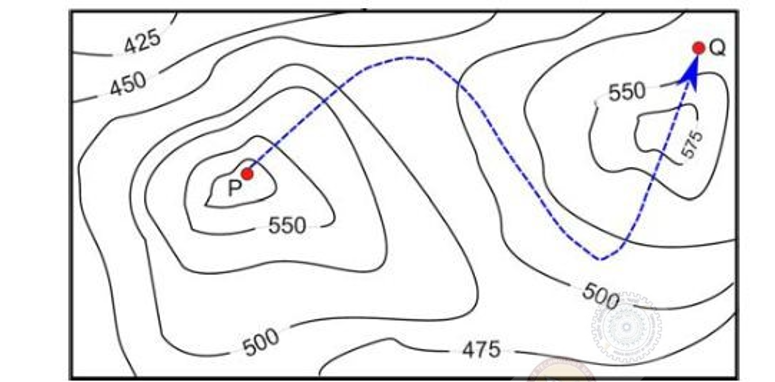
\includegraphics[width=0.8\columnwidth]{figs/contourplot.png}
\caption{Contour plot showing the path from P to Q}
\label{fig:contour_path}
\end{figure}

The path from P to Q is best described by
\begin{enumerate}
  \item Up--Down--Up--Down
  \item Down--Up--Down--Up
  \item Down--Up--Down
  \item Up--Down--Up
\end{enumerate}
\hfill (GATE BT 2017)
\end{enumerate}
\end{document}




 

